\documentclass{beamer}
\usepackage{ctex}
\usepackage{graphicx}
\usepackage{tikz}
\usepackage{amsmath}
\usepackage{pgfplots}
\usepackage{pgfplotstable}
\usepackage{subcaption}
\usetikzlibrary{angles,quotes}

\title{Uniswap 简明导论}
\author{怀菁}
\institute{武汉大学}
\date{\today}

\usetheme{Madrid}


\begin{document}

\frame{\titlepage}

\begin{frame}
    \frametitle{这是什么?}

    \centering
    \includegraphics[width=0.8\textwidth]{../notes/rugpull.jpeg}

\end{frame}

\begin{frame}
    \frametitle{Uniswap 简介}

    \begin{itemize}
        \item 一个去中心化交易协议
        \item V1 上线时间:2018年11月2日
        \item 恒定积自动做市商
        \item 去中心化交易所的奠基者和领军者
    \end{itemize}

    ~

    \centering
    \includegraphics[width=0.2\textwidth]{Uniswap-Logo.png}
\end{frame}

\begin{frame}
    \frametitle{中心化交易所的订单簿}

    \centering
    \includegraphics[width=0.5\textwidth]{../notes/订单簿示意图.jpg}
\end{frame}

\begin{frame}
    \frametitle{例子:可乐自动售货机}

    \begin{itemize}
        \item 机器中有 $x_0$ 瓶可乐与 $y_0$ 枚一元硬币
        \item 一瓶可乐 3 元
        \item 交易若干次后,机器中有 $x$ 瓶可乐与 $y$ 枚一元硬币
    \end{itemize}

    \begin{equation}
        3x + y = 3x_0 + y_0
    \end{equation}

    设 $k=3x_0+y_0$ ,有 $y=-3x+k$

    \begin{figure}[htbp]
        \centering
        \begin{tikzpicture}[scale=0.7]
            \draw[-latex] (0,0) -- (2.5,0) node[right] {$x$};
            \draw[-latex] (0,0) -- (0,4) node[above] {$y$};
            \draw[domain=0:1, thick, red] plot (\x, {-\x*3+3});
            \node[left] at (0,3) {$k$};
        \end{tikzpicture}
    \end{figure}
    
\end{frame}

\begin{frame}
    \frametitle{为可乐交易所添加流动性}

    向交易所中投放更多的可乐和硬币,得到 $k'>k$ 

    \begin{figure}[htbp]
        \centering
        \begin{tikzpicture}[scale=0.7]
            \draw[-latex] (0,0) -- (4,0) node[right] {$x$};
            \draw[-latex] (0,0) -- (0,7) node[above] {$y$};
            \draw[domain=0:1, thick, red] plot (\x, {-\x*3+3});
            \node[left] at (0,3) {$k$};
            \draw[domain=0:2, thick, blue] plot (\x, {-\x*3+6});
            \node[left] at (0,6) {$k'$};
            \draw[->] (0.5,1.5) -- (1.3,2);
        \end{tikzpicture}
    \end{figure}

    这个可乐交易所就是一个\textbf{恒定和自动做市商}(CSAMM)
\end{frame}

\begin{frame}
    \begin{columns}
        \frametitle{Uniswap 恒定积自动做市商}

        \begin{column}{0.5\textwidth}
            \begin{itemize}
                \item X :计价货币(Quote Currency)
                \item Y :基准货币(Base Currency)
                \item Y/X :交易对
                \item $x_0$ : X 的储备量
                \item $y_0$ : Y 的储备量
            \end{itemize}

            \begin{equation}
                xy=k 
            \end{equation}

            \begin{equation}
                p_X = \frac{y_1}{x_1} = \tan \theta
            \end{equation}
        \end{column}

        \begin{column}{0.5\textwidth}
            \begin{figure}[htbp]
                \centering
                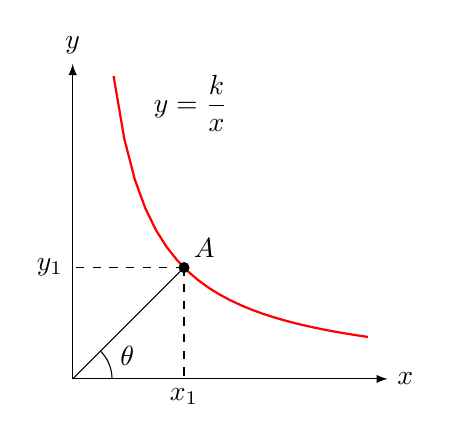
\begin{tikzpicture}
                    \draw[-latex] (0,0) -- (4,0) node[right] {$x$};
                    \draw[-latex] (0,0) -- (0,4) node[above] {$y$};
                    \draw[domain=0.52:3.75, thick, red] plot (\x, {2/\x});
            
                    \fill ({sqrt(2)},{sqrt(2)}) circle (2pt);
                    \node[above right] at ({sqrt(2)},{sqrt(2)}) {$A$};
            
                    \coordinate (A) at ({sqrt(2)},{sqrt(2)});
                    \coordinate (O) at (0,0);
                    \coordinate (B) at ({sqrt(2)},0);
                    \coordinate (C) at (0,{sqrt(2)});
                    \draw (A) -- (O);
                    \pic [draw, pic text=$\theta$, angle eccentricity=1.5] {angle = B--O--A};
            
                    \draw[dashed] (A) -- (B);
                    \draw[dashed] (A) -- (C);
                    \node[below] at (B) {$x_1$};
                    \node[left] at (C) {$y_1$};
            
                    \node at (1.5,3.5) {$\displaystyle y=\frac{k}{x}$};
                \end{tikzpicture}
                \caption{Y/X交易对储备图}
            \end{figure}
        \end{column}
    \end{columns}
\end{frame}

\begin{frame}
    \frametitle{交易改变价格}

    \begin{columns}
        \begin{column}{0.5\textwidth}
            假设交易者用 $\Delta x$ 个货币 X 购买一些货币 Y

            $$x'=x_0+\Delta x$$

            \begin{equation}
                x'y'=k
            \end{equation}

            \begin{equation}
                y' = \frac{k}{x'} = \frac{k}{x_0+\Delta x} < y_0
            \end{equation}

            交易者买到的 Y 的数量即为

            \begin{equation}
                \Delta y = y_0-y' = y_0 - \frac{k}{x_0+\Delta x}
            \end{equation}

        \end{column}

        \begin{column}{0.5\textwidth}
            \begin{figure}[htbp]
                \centering
                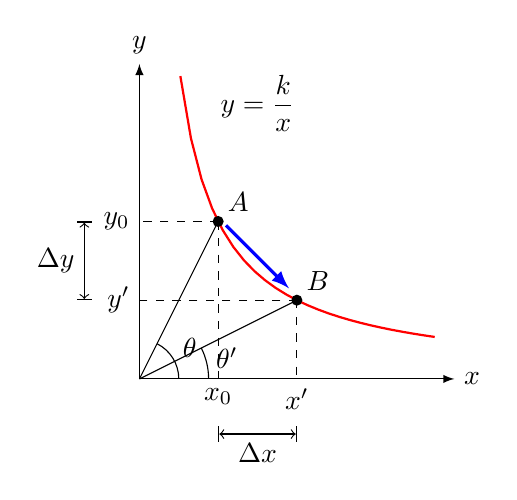
\begin{tikzpicture}[scale = 1]
                    \draw[-latex] (0,0) -- (4,0) node[right] {$x$};
                    \draw[-latex] (0,0) -- (0,4) node[above] {$y$};
                    \draw[domain=0.52:3.75, thick, red] plot (\x, {2/\x});
                    \node at (1.5,3.5) {$\displaystyle y=\frac{k}{x}$};
            
                    \coordinate (A) at (1,2);
                    \coordinate (O) at (0,0);
                    \coordinate (B) at (1,0);
                    \coordinate (C) at (0,2);
                    \fill (A) circle (2pt);
                    \node[above right] at (A) {$A$};
            
                    \draw (A) -- (O);
                    \pic [draw, pic text=$\theta$, angle eccentricity=1.5] {angle = B--O--A};
            
                    \draw[dashed] (A) -- (B);
                    \draw[dashed] (A) -- (C);
                    \node[below] at (B) {$x_0$};
                    \node[left] at (C) {$y_0$};
            
                    
                    \coordinate (D) at (2,1);
                    \coordinate (E) at (2,0);
                    \coordinate (F) at (0,1);
                    \fill (D) circle (2pt);
                    \node[above right] at (D) {$B$};
            
                    \draw (D) -- (O);
                    \pic [draw, pic text=$\theta'$, angle eccentricity=1.3, angle radius=25] {angle = E--O--D};
                    
                    \draw[dashed] (D) -- (E);
                    \draw[dashed] (D) -- (F);
                    \node[below] at (E) {$x'$};
                    \node[left] at (F) {$y'$};
            
                    \draw[-latex, very thick, blue] (1.1,1.95) -- (1.9,1.15);
                    \draw[|<->|] (1,-0.7) -- node[below] {$\Delta x$} (2,-0.7);
                    \draw[|<->|] (-0.7,1) -- node[left] {$\Delta y$} (-0.7,2);
            
                \end{tikzpicture}
                \caption{交易改变了价格}
            \end{figure}
        \end{column}
    \end{columns}
\end{frame}

\begin{frame}
    \frametitle{添加或移除流动性}

    \begin{columns}
        \begin{column}{0.5\textwidth}
            流动性提供者(Liquidity Provider)为流动性池提供资金,并赚取交易手续费。
            
            $$x'=x_1+x_2,y'=y_1+y_2$$

            $$k'=x'y'$$

            那么新的恒定积公式就是

            $$xy = k'$$
        \end{column}

        \begin{column}{0.5\textwidth}
            \begin{figure}[htbp]
                \centering
                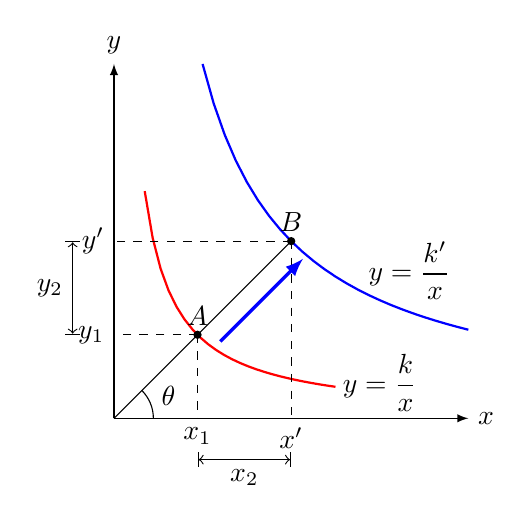
\begin{tikzpicture}[scale=0.75]
                    \draw[-latex] (0,0) -- (6,0) node[right] {$x$};
                    \draw[-latex] (0,0) -- (0,6) node[above] {$y$};
                    \draw[domain=0.52:3.75, thick, red] plot (\x, {2/\x});
                    \draw[domain=1.5:6, thick, blue] plot (\x, {9/\x});
            
                    \coordinate (A) at ({sqrt(2)},{sqrt(2)});
                    \coordinate (O) at (0,0);
                    \coordinate (B) at ({sqrt(2)},0);
                    \coordinate (C) at (0,{sqrt(2)});
                    \coordinate (D) at (3,3);
                    \coordinate (E) at (3,0);
                    \coordinate (F) at (0,3);
            
                    \fill (A) circle (2pt);
                    \node[above] at (A) {$A$};
                    \fill (D) circle (2pt);
                    \node[above] at (D) {$B$};
            
                    \draw (D) -- (O);
                    \pic [draw, pic text=$\theta$, angle eccentricity=1.5] {angle = B--O--A};
            
                    \draw[dashed] (A) -- (B);
                    \draw[dashed] (A) -- (C);
                    \node[below] at (B) {$x_1$};
                    \node[left] at (C) {$y_1$};
            
                    \draw[dashed] (D) -- (E);
                    \draw[dashed] (D) -- (F);
                    \node[below] at (E) {$x'$};
                    \node[left] at (F) {$y'$};
            
                    \node at (4.5,0.6) {$\displaystyle y=\frac{k}{x}$};
                    \node at (5,2.5) {$\displaystyle y=\frac{k'}{x}$};
                    
                    \draw[-latex, very thick, blue] (1.8,1.3) -- (3.2,2.7);
                    \draw[|<->|] ({sqrt(2)},-0.7) -- node[below] {$x_2$} (3,-0.7);
                    \draw[|<->|] (-0.7,{sqrt(2)}) -- node[left] {$y_2$} (-0.7,3);
            
                \end{tikzpicture}
                \caption{添加流动性引起储备曲线缩放}
            \end{figure}
        \end{column}
    \end{columns}
\end{frame}

\begin{frame}
    \frametitle{添加流动性的好处}

    \begin{itemize}
        \item 降低交易者的滑点(Slippage)
        \begin{equation}
            \left| \frac{\Delta x}{\Delta y} - \frac{x_0}{y_0} \right|
             = \left| \frac{\Delta x}{y_0} \right|
        \end{equation}
        \item 减弱价格推动效应
        \begin{equation}
            |p_X'-p_X| = \left| \frac{x_0y_0}{(x_0+\Delta x)^2} - \frac{y_0}{x_0} \right| = \left| \frac{2x_0y_0\Delta x - y_0(\Delta x)^2}{x_0(x_0+\Delta x)^2} \right|
        \end{equation}
    \end{itemize}
\end{frame}

\begin{frame}
    \frametitle{收益分配的依据:流动性代币}

    流动性代币(Liquidity Token)是一种特殊的代币,它衡量了 LP 对流动性池的贡献。它是所有者权益的凭证,或者简单理解为流动性池的股票。

    \begin{itemize}
        \item LP 存入 X 和 Y 时,流动性池铸造一种名为“YX”的代币发送给 LP 
        \item LP 将 YX 发送至流动性池销毁掉,就可以按份额提取出自己的 X 和 Y 
    \end{itemize}
    
    对于第一位 LP ,其获得的流动性代币数量为

    \begin{equation}
        s = \sqrt{x_0y_0}
    \end{equation}

    对于之后的 LP ,其获得的流动性代币数量为

    \begin{equation}
        \Delta s = \frac{x_1}{x_0} s_0 = \frac{y_1}{y_0} s_0
    \end{equation}

    并使用 $s_0 \leftarrow s_0 + \Delta s$ 更新 $s_0$ 的值
\end{frame}

\begin{frame}
    \frametitle{风险1:流动性不足——三明治攻击}

    \begin{table}[htbp]
        \centering
        \begin{tabular}{lll}
            & 价格  & 数量 \\ \hline
            卖2 & 1.2 & 1  \\ \hline
            卖1 & 0.9 & 1 
        \end{tabular}
    \end{table}

    订单簿中的三明治攻击:经纪商买入 -> 经纪商挂卖单 -> 交易者买入

    \begin{figure}
        \centering
        \includegraphics[width=\textwidth]{../notes/三明治攻击示意图.png}
    \end{figure}

    AMM 中的三明治攻击:攻击者买入 -> 交易者买入 -> 攻击者卖出

    ~

    \begin{itemize}
        \item 都是依靠自己的单边信息优势,获取无风险利润
        \item 提高流动性可以使这种攻击无利可图
    \end{itemize}
    
\end{frame}

\begin{frame}
    \frametitle{风险1:流动性不足——撤池跑路}

    撤池跑路(Rug Pull)是指 LP 突然撤出全部的流动性使交易者无法再交易的行为

    \begin{figure}
        \centering
    \includegraphics[width=0.8\textwidth]{../notes/rugpull.jpeg}
    \end{figure}

    锁仓可以降低 Rug Pull 风险

\end{frame}

\begin{frame}
    \frametitle{风险2:无常损失}

    \begin{itemize}
        \item 恒定积自动做市商存在着“劣币驱逐良币”的倾向
        \item 这意味着更有价值的货币将持续流出
        \item 而劣币的占比和绝对数额将会提高
        \item LP 可能因此受到财产损失
    \end{itemize}

    \begin{equation}
        \begin{matrix}
            \left\{ 
                \begin{aligned}
                    & X/USD = a_0 \\
                    & Y/USD = b_0 \\
                    & Y/X = \frac{x_0}{y_0}\\
                    & x_0y_0 = k
                \end{aligned}
            \right.
            & \rightarrow &
            \left\{ 
                \begin{aligned}
                    & X/USD = a_1 \\
                    & Y/USD = b_1 \\
                    & Y/X = \frac{x_1}{y_1}\\
                    & x_1y_1 = k
                \end{aligned}
            \right.
        \end{matrix}
    \end{equation}

    \begin{equation}
    r = \frac{B_1}{B_0} 
    = \frac{a_1x_1+b_1y_1}{a_0x_0+b_0y_0} 
    = \frac{\sqrt{a_1b_1}}{\sqrt{a_0b_0}}
    \end{equation}

    \begin{equation}
        r^* = \frac{B^*}{B_0} = \frac{a_1x_0+b_1y_0}{a_0x_0+b_0y_0}
    \end{equation}
\end{frame}

\begin{frame}
    \frametitle{风险2:无常损失}

    无常损失(Impermanent Loss)是由于流动性池中两种代币的\textbf{相对}价格变化导致的、相较于单纯持有代币的机会损失
    
    \begin{columns}
        \begin{column}{0.6\textwidth}
            \begin{equation}
                \begin{aligned}
                    \delta 
                    & = r - r^*  \\ 
                    & = \frac{a_1(x_1-x_0) + b_1(y_1-y_0)}{a_0x_0 + b_0y_0} \\
                    & = \frac{2\sqrt{a_1b_1} - \left( a_1\sqrt{\frac{b_0}{a_0}} + b_1\sqrt{\frac{a_0}{b_0}} \right)}{2\sqrt{a_0b_0}} \\
                    & \le \frac{2\sqrt{a_1b_1} - 2\sqrt{a_1\sqrt{\frac{b_0}{a_0}} \cdot b_1\sqrt{\frac{a_0}{b_0}}}}{2\sqrt{a_0b_0}} \\
                    & = \frac{2\sqrt{a_1b_1} - 2\sqrt{a_1b_1}}{2\sqrt{a_0b_0}} \\
                    & = 0
                \end{aligned}
            \end{equation}
        \end{column}

        \begin{column}{0.4\textwidth}
            当且仅当 $\displaystyle a_1\sqrt{\frac{b_0}{a_0}} = b_1\sqrt{\frac{a_0}{b_0}}$ 即 $\displaystyle \frac{a_0}{b_0} = \frac{a_1}{b_1}$ 时取等号

            \begin{itemize}
                \item 也就是说只要相对价格与初始相对价格不一致,就会产生无常损失
                \item 而当二者回归一致时,无常损失就为 0 
            \end{itemize}

        \end{column}
    \end{columns}
\end{frame}

\begin{frame}
    \frametitle{风险2:无常损失}

    当 $a_0=b_0$ 时,无常损失的图像与 $z=0$ 平面相切于 $y=x$ 直线

    \begin{figure}
        \centering
        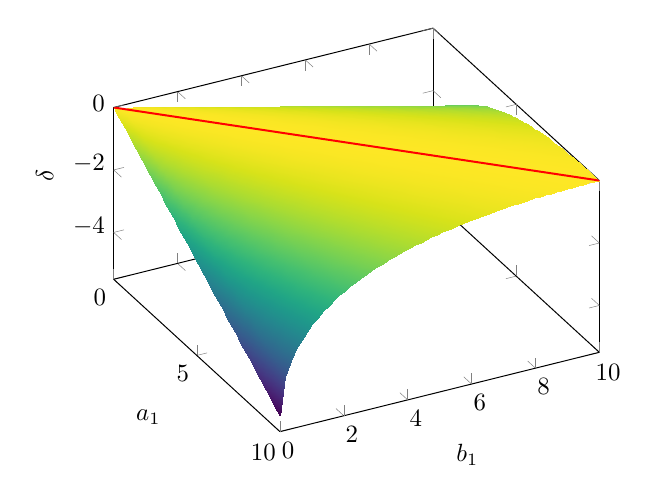
\begin{tikzpicture}[scale=0.9]
            \begin{axis}[
              xlabel={$a_1$},
              ylabel={$b_1$},
              zlabel={$\delta$},
              domain=0:10,
              domain y=0:10,
              view={62.5}{45},
              zmax=0,
            ]
          
            \addplot3[surf, colormap/viridis, shader=interp, samples=60] {(2*sqrt(x*y) - (x + y))/2};
    
            \addplot3[domain=0:10, samples=2, samples y=0, red, thick] ({x}, {x}, 0);
          
            \end{axis}
        \end{tikzpicture}
        \caption{无常损失 $\delta$ 图像}
    \end{figure}
\end{frame}

\begin{frame}
    \frametitle{风险3:诈骗、假币与洗钱犯罪}

    任何人都可以创建假的 USDT 、BTC 和 ETH 代币并建立流动性池

    ~

    利用 Uniswap 进行洗钱犯罪难以追查

\end{frame}

\begin{frame}
    \frametitle{风险4:价格预言机失灵}

    \begin{itemize}
        \item 预言机(Oracle)使得链上合约可以读取链下信息,比如某个代币的价格
        \item 因为套利者的存在, Uniswap 可以扮演价格预言机,但早期版本容易被操纵
        \item V2 更新:在每一个区块开始就计算并确定报价,此后的交易改变实时价格,但不再改变报价,从而保证报价的相对稳定性
    \end{itemize}

\end{frame}

\begin{frame}
    \frametitle{风险5:黑客攻击}

    \begin{itemize}
        \item 屎山代码,bug 连篇
        \item 留下后门,监守自盗
        \item Uniswap V2 将存放资金的“核心合约”与实现其他功能的“边缘合约”分隔开,从而最小化攻击面
    \end{itemize}
\end{frame}

\begin{frame}
    \frametitle{新特性:集中流动性}

    缩小价格值域,只给某一个区间提供流动性,而不是整个正实数域

    \begin{figure}
        \centering
        \begin{tikzpicture}
            \draw[-latex] (0,0) -- (4,0) node[right] {$x$};
            \draw[-latex] (0,0) -- (0,4) node[above] {$y$};
            
            \draw[domain=0.28:3.5, red, thick] plot (\x, {1/\x});
            \draw[domain=0:1.5, blue, thick] plot (\x, {1/(\x+0.5)-0.5});
    
            \draw[-latex, blue, thick] (0.95,0.95) -- (0.55,0.55);
        \end{tikzpicture}
        \caption{集中流动性使储备曲线平移}
    \end{figure}

\end{frame}

\begin{frame}
    \frametitle{新特性:单例和闪电记账}

    \begin{itemize}
        \item 单例(Singleton):使用一个合约管理链上所有的流动性池
        \item 闪电记账(Flash Accounting):多重交换的过程只需要支付资金进出系统的两次 gas fee
    \end{itemize}

    \begin{figure}[htbp]
        \centering
        \includegraphics[width=12cm]{../notes/闪电记账示意图.jpg}
        \caption{闪电记账示意图}
    \end{figure}
\end{frame}

\begin{frame}
    \frametitle{新特性:挂钩}

    \begin{itemize}
        \item 挂钩(Hooks):一个与流动性池相匹配的外部合约,其中实现了当流动性池在特定时间检查是否满足特定条件,并执行相应操作
        \item 特定时间包括:初始化、调整持仓、交换和支付的之前和之后
    \end{itemize}

    \begin{figure}[htbp]
        \centering
        \includegraphics[width=6cm]{../notes/Hooks.png}
        \caption{挂钩示意图}
    \end{figure}
\end{frame}

\begin{frame}
    \frametitle{结论与思考讨论}

    \begin{enumerate}
        \item 了解了 Uniswap 的利弊之后,你是更愿意选择中心化交易所还是去中心化交易所?为什么?
        \item 交易费过高会提升交易者的交易成本,过低又会打击 LP 的积极性。你认为什么水平的交易费才是最合适的?你是根据什么原则来确定交易费水平的?
        \item 在你看来,相较于旧版的多池,单例模式是否违背了 Web3 去中心化的核心价值观?用一个合约管理所有的流动性池会造成多大的风险?这种风险相比于它带来的方便性是值得我们去承担的吗?
        \item 从宏观经济角度来看,为了保持交易所的流动性,社会总是需要在流动性池中锁定一笔价值不菲的资金。在你看来,这笔资金应当被视为储蓄还是投资?假如一个实力雄厚的巨鲸(或者称之为“政府”)向流动性池注入大笔资金,会对经济系统造成什么影响?
        \item 你认为还有哪些值得思考的问题?
    \end{enumerate}
\end{frame}

\begin{frame}
    \centering \Huge
    \emph{Thanks for Listening!}
\end{frame}

\end{document}